\newpage
\section{Group-sparse logistic regression}

Finally, we would like to highlight our progress in extending the methodology to the setting of binary classification. Generally, variational inference within this setting requires greater care than the linear counterpart, this is because there is no closed form for the expectation of the log-likelihood under the variational family. 

Several authors have proposed bounds or approximations to maintain tractability. Notably, \cite{Depraetere2017a} compared several different approximations and bounds. Their results highlight that quadratic bounds do not perform well, and  Taylor series approximations are only accurate in specific settings. They conclude that non-quadratic bounds can perform well, and approximations based on quasi-Monte Carlo, as proposed by the authors performs better, albeit slower, in their simulations. Finally, the authors note, a potential avenue for future research is producing tighter bounds or faster approximations, e.g. through a combination of methods. Ultimately pursuing an improvement the variational approximation both in terms of accuracy and computation time. 
% \red{cite a few people e.g. JJ99, KM13 etc.}.

\subsection{Problem formulation}

Formally, we are going to be modelling a binary response $Y \in \{0, 1 \}$ alongside a feature vector $x \in \R^p$, by using the popular logistic link function wherein,
\begin{equation}
    \P(Y = 1 | X = x) = \logistic(x^\top \beta) =  \frac{\exp(x^\top \beta)}{1 + \exp(x^\top \beta)}
\end{equation}
where $\beta \in \R^p$ is the coefficient vector. Wherein the log-likelihood,
\begin{equation}
    \ell(\D, \beta) 
    % =&\ \sum_{i=1}^n 
	% y_i \log \left( \frac{ \exp(x_i^\top \beta) }{ 1 + \exp( x_i^\top \beta ) } \right) +
	% (1 - y_i) \log \left( \frac{ 1 }{ 1 + \exp( x_i^\top \beta ) } \right) \nonumber \\
    % =&\ 
    = 
	\sum_{i=1}^n  y_i \left( x_i^\top \beta \right) 
	- \log \left(1 + \exp(x_i^\top \beta) \right)
\end{equation}
where we denote the training data $\D = \{(y_i, x_i)\}_{i=1}^n$ with $y_i \in \{0, 1\}, x_i \in \R^p$. Further, we denote, $y=(y_1, \dots, y_n)^\top$ and $X=(x_1, \dots, x_n)^\top \in \R^{n \times p}$. 
% We are going to assume that the group structure is known. We will be using the same notation introduced earlier for the groups. 

Just like in the linear case we are aiming to minimize
\begin{equation} \label{eq:l_opt_objective} 
    \E_Q \left[ 
	- \ell(\D; \beta) + \log \frac{dQ}{d\Pi}(\beta) 
    \right]
\end{equation}
with respect to the parameters of the variational family, chosen as,
\begin{equation}
    \Q =
    \left\{ \Theta(\mu, \sigma, \gamma) = 
	\bigotimes_{k=1}^M 
	\left[ 
	    \gamma_k\ N\left(\mu_{G_k}, \diag(\sigma_{G_k}^2) \right) + 
	    (1-\gamma_k) \delta_0
	\right] 
    \right\} \\
\end{equation}
Note, unlike our previous variational family, we do not need to model $\tau^2$, and hence drop the component of this term from the variational family.

\subsection{A new bound}

In light of the suggestions by \cite{Depraetere2017a}, we propose a non-quadratic bound based on the inequality 
\begin{equation} \label{eq:logistic_bound}
\log(1 + \exp(x)) \leq \frac{1}{2} \left( x + \sqrt{2 + x^2} \right)
\end{equation}
% A comparison presented in \Cref{fig:bounds_comparison} indicates the bound is tight, particularly around the origin.
% \begin{figure}[htp]
%     \centering
%     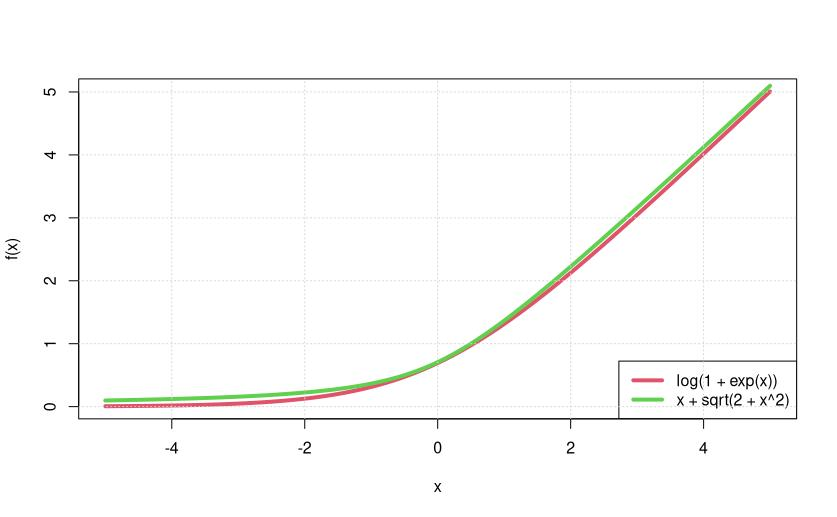
\includegraphics[width=\textwidth]{./figures/bounds.jpg}
%     \caption{Comparison to bound}
%     \label{fig:bounds_comparison}
% \end{figure}

% \section{Co-ordinate ascent update equations}
Meaning we can upper bound the expectation of the negative log-likelihood as
% \begin{equation} \label{eq:l_objective} 
%     \sum_{i=1}^n  
%     \E \left[
% 	    \log \left(1 + \exp(x_i^\top \beta) \right) -
% 	    y_i \left( x_i^\top \beta \right) 
%     \right]
% \end{equation}
% We note the first term is intractable and therefore propose bounding it using the fact that
\begin{align*}
    \E \left[ \log(1 + \exp(x_i^\top \beta)) \right]
    \leq &\
	\E \left[ 
	    \frac{1}{2} \left( x_i^\top \beta + 
	    \sqrt{2 + (x_i^\top \beta)^2} \right) 
	\right] \\
    \leq &\
	\frac{1}{2} \left( 
	    \E \left[ x_i^\top \beta \right] + 
	    \sqrt{2 + \E \left[(x_i^\top \beta)^2 \right]} 
	\right)
\end{align*}
where the first inequality follows form \eqref{eq:logistic_bound} and the second inequality from Jensen's inequality. Hence,
\begin{equation}
    \sum_{i=1}^n
    \left( \frac{1}{2} - y_i \right) \E \left[ x_i^\top \beta \right] + 
    \frac{1}{2} \left( 2 + \sum_{j=1}^p \sum_{k=1}^p x_{ij} x_{ik} 
    \E \left[ \beta_j \beta_k \right] \right)^{1/2}
\end{equation}

Early simulation results have indicated that the bound is not tight enough and does not perform well. 

\subsection{Bound using Jensen's inequality}

Bounding the likelihood using Jensen's inequality is straightforward,
\begin{align}
    \E_Q \left[ - \ell(\D; \beta) \right]
    =&\ 
	\sum_{i=1}^n  \E_Q \left[
	    \log \left(1 + \exp(x_i^\top \beta) \right) 
	    -
	    y_i \left( x_i^\top \beta \right) 
	\right] 
    \nonumber \\
    \leq &\ 
	\sum_{i=1}^n  
	    \log \left(1 + \E_Q \left[ \exp(x_i^\top \beta) \right] \right) 
	    -
	    y_i \sum_{k=1}^M \gamma_k \sum_{j \in G_k} x_{ij} \mu_{j}
    \label{eq:logistic_jensens}
\end{align}
where
\begin{equation*}
    \E_Q \left[ \exp(x_i^\top \beta) \right]
    =	
	\prod_{k=1}^M \gamma_k \exp \left\{ 
	    \sum_{j \in G_k} 
	    x_{ij} \mu_{j}
	    + 
	    \frac{1}{2} x_{ij}^2 \sigma_{j}^2
	\right\}
	+
	(1- \gamma_k)
\end{equation*}
Based on \eqref{eq:logistic_jensens} it is straightforward to derive the update equations for $\mu_{G_k}, \sigma_{G_k}$ and $\gamma_k$.


\subsection{Bound based on \cite{Jakkola97}}

\cite{Jakkola97} introduce a quadratic bound for the sigmoid function $\sigmoid(x) = (1 + \exp(-x))^{-1}$, given as
\begin{equation} \label{eq:jj_bound}
    \sigmoid(x) 
    \geq 
	\sigmoid(t)
	\exp \left\{
	    \frac{x-t}{2}
	    -
	    \frac{a(t)}{2} (x^2 - t^2)
	\right\}
\end{equation}
where $a(t) = \frac{\sigmoid (t) - 1/2}{t}$ and $t$ is a variational parameter that must be optimized to ensure the bound is tight.

Using the fact that $\P(Y=y_i | X=x_i)$ can be written as $e^{y_i x_i^\top \beta} \sigmoid(- x_i^\top \beta)$, we have
\begin{align}
    - \ell(\D; &\ \beta)
    = 
	\sum_{i=1}^n  
	    - y_i x_i^\top \beta 
	    - \log \sigmoid (-x_i^\top \beta)
    \nonumber \\
    \leq &\
	\sum_{i=1}^n  
	    - y_i x_i^\top \beta 
	    - \log \sigmoid (t_i)
	    + \frac{x_i^\top \beta + t_i}{2}
	    + \frac{a(t_i)}{2} ((x_i^\top \beta)^2 - t_i^2)
    \nonumber \\
    = &\ 
	- \langle y,  X^\top \beta \rangle 
	- \langle 1, \log s(t) \rangle
	+ \frac{1}{2} \left(
	    \langle 1, X^\top \beta + t \rangle
	    + \beta^\top X^\top A_t X \beta 
	    - t^\top A_t t
	\right)
    \label{eq:jj_likelihood}
\end{align}
where $t_i$ is a variational parameter for each observation, $t=(t_1, \dots, t_n)^\top$, $A_t =\diag(a(t_i), \dots, a(t_n))$, $s(t) = (s(t_1), \dots, s(t_n))^\top$, and operators to vectors are performed element-wise, e.g. $\log s(t) = (\log s(t_i))_{i=1}^n$. Combining \eqref{eq:jj_likelihood} with results seen in the linear regression setting, it is straightforward to obtain the necessary update equations. 

Taking the expectation of \eqref{eq:jj_likelihood} wrt. $Q$, gives,
\begin{equation} \label{eq:jj_expectation_Q} 
\begin{aligned}
    \left(
    \sum_{k = 1}^M 
	\gamma_k \langle 1/2 - y,  X_{G_k} \mu_{G_k} \rangle 
    \right) 
    +
    \frac{1}{2}
    \left(
	\sum_{i,j=1}^p 
	    (X^\top A_t X)_{ij} \E_Q [ \beta_i \beta_j ]
    \right)
    - 
    \frac{t^\top A_t t}{2}
    \\
    + \langle 1, t/2 - \log s(t) \rangle
\end{aligned}
\end{equation}

Updates for $\mu_{G_k}$ and $\sigma_{G_k}$ are given by finding the minimizers of 
\begin{equation}
\begin{aligned}
    & 
    \langle 1/2 - y,  X_{G_k} \mu_{G_k} \rangle 
    + \frac{1}{2} \left( 
	\mu_{G_k}^\top X_{G_k}^\top A_t X_{G_k} \mu_{G_k} 
	+ \sum_{i \in G_k} (X^\top A_t X)_{ii} \sigma_{i}^2 
	% - t^\top A_t t
    \right)
    \\
    & 
    + \sum_{j \neq k} \gamma_j \mu_{G_k}^\top X_{G_k}^\top A_t X_{G_j} \mu_{G_j} 
    % + \langle 1, t/2 - \log s(t) \rangle
    + \lambda \left( \sigma_{G_k}^\top \sigma_{G_k} + \mu_{G_k}^\top \mu_{G_k} \right)^{1/2} 
    - \sum_{i \in G_k}\log{\sigma_i}
    % + C
\end{aligned}
\end{equation}
Updates for $\gamma_k$
\begin{equation}
\begin{aligned}
    \log &\ \frac{\gamma_K}{1-\gamma_K} = 
    \log \frac{\bar{w}}{1-\bar{w}}
    + \frac{m_K}{2}  
    + \langle y - 1/2, X_{G_K} \mu_{G_K} \rangle  
    % + \langle 1,\log s(t) - t/2 \rangle
    \\
    &
    + \frac{1}{2} \sum_{j \in G_K} \log \left( 2 \pi \sigma_j^2 \right)
    + \log(C_K)
    + m_K \log (\lambda)
    - \Bigg\{ 
    \lambda \left( \sum_{i \in G_K} \sigma_i^2 + \mu_i^2 \right)^{1/2}  
    % - \frac{t^\top A_t t}{2}
    \\
    &
    + \frac{1}{2} \left( 
	\mu_{G_k}^\top X_{G_k}^\top A_t X_{G_k} \mu_{G_k} 
	+ \sum_{i \in G_k} (X^\top A_t X)_{ii} \sigma_{i}^2 
    \right)
    + \sum_{j \neq k} \gamma_j \mu_{G_k}^\top X_{G_k}^\top A_t X_{G_j} \mu_{G_j} 
\Bigg\}
\end{aligned}
\end{equation}
ELBO given by combining the negation of \eqref{eq:jj_expectation_Q} and $\E_Q[ - \log dQ / d\Pi]$,
\begin{equation}
\begin{aligned}
\L_Q(\D) =
    &\
    \frac{1}{2}
    \left(
	t^\top A_t t
	- \sum_{i,j=1}^p (X^\top A_t X)_{ij} \E_Q [ \beta_i \beta_j ]
    \right)
    - \left(
    \sum_{k = 1}^M 
	\gamma_k \langle 1/2 - y,  X_{G_k} \mu_{G_k} \rangle 
    \right) 
    \\
    &
    - \langle 1, t/2 - \log s(t) \rangle
    + \sum_{k=1}^M \bigg(  
	\frac{\gamma_k}{2} \sum_{j \in G_k} \left( \log( 2 \pi \sigma_j^2) \right)
	+ \gamma_k \log(C_k)
	+ \frac{\gamma_k m_k}{2} 
    \\
    &
	+ \gamma_k m_k \log (\lambda)
	- \E_Q \left[ \I_{z_k =1} \lambda \| \beta_{G_k} \| \right]
	- \gamma_k \log \frac{\gamma_k}{\bar{w}}
	- (1-\gamma_k) \log \frac{1 - \gamma_k}{1 - \bar{w}} 
    \bigg)
\end{aligned}
\end{equation}

Updates for $t_i$ are found by maximizing the ELBO, and are given by
\begin{equation}
    t_i = \left( 
	\sum_{k=1}^M \gamma_k \left[
	    (\mu_{G_k}^\top x_{i, G_k})^2 + \sum_{j \in G_k} \sigma_{j}^2 x_{i, j}^2
	\right]
    \right)^{1/2}
\end{equation}


\subsection{A new bound \#2}

Here we derive a new bound by introducing variational parameters to tighten the bound based on Jensen's inequality. Formally, we write,
\begin{equation} \label{eq:new_bound_2}
    -\log s(-x) 
    = \log \left\{ e^{x t} \left( e^{-x t} + e^{x - x t} \right) \right\}
    = x t + \log \left( e^{-x t} + e^{x - x t} \right)
\end{equation}
where $t$ is a variational parameter that needs to be optimized. We then bound the expectation of the \eqref{eq:new_bound_2} using Jensen's,
\begin{equation}
    -\E \log s(-x)
    \leq
    \E \left[ x t_i \right] + \log \E \left[ e^{-x t} + e^{(1-t)x} \right]
\end{equation}
Hence
\begin{equation}
    \E_Q \ell (\D; \beta) 
    \leq 
    \sum_{i=1}^n 
    \left( \sum_{k=1}^M \gamma_k (t_i - y_i) x^\top_i \mu_{G_k} \right)
    +
    \log \E_Q \left[ e^{-t_i x_i^\top \beta} + e^{(1-t_i)x_i^\top \beta} \right]
\end{equation}
where
\begin{equation*}
    \E_Q \left[ \exp(a x_i^\top \beta) \right]
    =	
	\prod_{k=1}^M \gamma_k \exp \left\{ 
	    \sum_{j \in G_k} 
	    a x_{ij} \mu_{j}
	    + 
	    \frac{1}{2} a^2 x_{ij}^2 \sigma_{j}^2
	\right\}
	+
	(1- \gamma_k)
\end{equation*}
for $a \in \R$.

A new bound 2 is not so good


\subsection{A new bound \#3}

We introduce a new bound. Formally, let $\X \sim N(\mu, \sigma^2)$, then
\begin{equation} \label{eq:new_tight}
\begin{aligned}
    \E_\X \left[ \log(1 + \exp(x)) \right] \leq
	\frac{\sigma}{\sqrt{2\pi}} e^{- \frac{\mu^2}{2 \sigma^2}}
	+ \mu \Phi \left(\frac{\mu}{\sigma} \right)
	+ e^{\mu + \sigma^2 / 2 }  \Phi \left( -\frac{\mu}{\sigma} - \sigma \right) \\
	+ e^{-\mu + \sigma^2 /2 } \Phi \left( \frac{\mu}{\sigma} - \sigma \right)
\end{aligned}
\end{equation}

\textit{Proof.} Write $\boldsymbol{Z} = \X - \mu$ and denote the density of $\boldsymbol{Z}$ as $\phi_z$. It follows that,
{\allowdisplaybreaks %
\begin{align}
    \E_{\boldsymbol{X}} [ \log(1 & + \exp(x)) ] =
    \E_{\boldsymbol{Z}} [ \log(1+ \exp(z + \mu)) ]
    \nonumber
    \\
    =&\ 
	\int_{-\mu}^\infty \log(1 + \exp(z + \mu)) \phi_z dz
	+ \int_{-\infty}^{-\mu} \log(1 + \exp(z + \mu)) \phi_z dz
    \nonumber
    \\
    =&\ 
	\int_{-\mu}^\infty (z + \mu) \phi_z  
	+ \int_{-\mu}^\infty + \log[1 + \exp(-(z+\mu))] \phi_z dz 
    \nonumber \\
    +&\ \int_{-\infty}^{-\mu} \log(1 + \exp(z + \mu))\phi_z dz
    \nonumber
    \\
    \leq &\ 
	\int_{-\mu}^\infty (z + \mu) \phi_z  
	+ \int_{-\mu}^\infty \exp(-(z+\mu)) \phi_z dz 
	+ \int_{-\infty}^{-\mu} \exp(z + \mu)) \phi_z dz
    \nonumber
\end{align}%
} %
where the inequality follows from $\log(1+x) \leq x$ for $x \in [0, 1]$, and \eqref{eq:new_tight} follows from the fact that $\phi(z)' = - z\phi(z) / \sigma^2 $ and $ \int_{a}^b e^{tz} \phi_z dz = e^{\sigma^2 t^2 / 2} \left[ \Phi(b/\sigma - t \sigma) - \Phi(a/\sigma - t\sigma) \right]$. $\qed$

Comparing our new bound and the bound introduced by \citep{Jakkola97}, against the value computed using quadrature (\Cref{fig:bound_comp}), we notice our new bound is orders of magnitude better, expect for the when the mean and standard deviation is are small.
\begin{figure}[hb]
    \centering
    \includegraphics[width=\textwidth]{./figures/comp_new_bound.pdf}
    \caption{Comparison of bound against \citep{Jakkola97}}
    \label{fig:bound_comp}
\end{figure}

Finally, to employ the bound in the context of our spike-and-slab variational family, we note that, $\E_Q \log ( 1 + \exp (x_i^\top \beta))$ can be written as,
\begin{equation} \label{eq:ll_expectation}
    \sum_{s \in S} \left( 
	\prod_{k=1}^M \gamma_k^{s_k} (1- \gamma_k )^{1- s_k} 
    \right)
    \E_{\underset{j \in J_s}{\otimes} N_j}
    \left( 
	\log \left[ 1 + \exp \left( \sum_{j \in J} x^\top_{i, G_j} \beta_{G_j} \right) \right] 
    \right)
\end{equation}
where $ S = \{0, 1\}^{M}$ and $J_s = \{j : s_j = 1, j=1,\dots,M \}$. Evidently, there are $2^M$ terms in \eqref{eq:ll_expectation}, meaning for large $M$ the expression is computationally intractable. To work around this limitation, recall, we are assuming there is sparsity in the true coefficient vector, therefore many of the $\gamma_k$s will be close to zero and few will be close to one, meaning \eqref{eq:ll_expectation} can be approximated by
\begin{equation}
    \E_{\underset{k \in K}{\otimes} N_k}
    \left( 
	\log \left[ 1 + \exp \left( \sum_{k \in K} x^\top_{i, G_k} \beta_{G_k} \right) \right] 
    \right)
\end{equation}
where $K = \{k : \gamma_k \geq t \}$ for some threshold $t$.




